
% ------------------------------------------------------------
% ------------------------------------------------------------

%%%%%%%%%%%%%%%%%%%%%%%%%%%%%%%%%%%%%
\section{Simulation Plots}
\subsection{Preliminaries}
%_______________________

\begin{frame}[fragile]
\frametitle{Simulations}
\framesubtitle{Preliminaries: The function \ttfamily outer() \normalfont}

    \begin{columns}[Tc]
      \column{0.42\textwidth}
\begin{lstlisting}
x=5:6; y=1:3
outer(x,y)
\end{lstlisting}

\begin{beamerboxesrounded}[shadow=true]{}
\ttfamily
\begin{verbatim}
     [,1] [,2] [,3] 
[1,]    5   10   15 
[2,]    6   12   18 
\end{verbatim}
\end{beamerboxesrounded}
\normalfont

	     \column{0.58\textwidth}
\begin{lstlisting}
fcn<-function(x,y){z=x+y}
outer(x,y,fcn)
\end{lstlisting}

\begin{beamerboxesrounded}[shadow=true]{}
\ttfamily
\begin{verbatim}
     [,1] [,2] [,3] 
[1,]    6    7    8 
[2,]    7    8    9 
\end{verbatim}
\end{beamerboxesrounded}
\normalfont
	\end{columns}
\end{frame}

%%%%%%%%%%%%%%%%%%%
\subsection{Performing the Simulation and Visualizing the Results}
%________________________________
\begin{frame}[fragile]
\frametitle{Simulations}
Suppose we want to know what the function $y\times sin(x)$ looks like:

\begin{lstlisting}
# Sample from the random uniform:
x <- sort(runif(100, min=0, max=10))
y <- x+runif(1)
f <- function(x,y) { r <- y*sin(x)}
z <- outer(x,y,f)
persp(x, y, z, col = "lightblue", shade = 0.1, ticktype = "detailed", expand=0.7)
\end{lstlisting}
\end{frame}

%______
\begin{frame}[fragile]
\frametitle{Simulations}
   \begin{figure}[ht]
       \begin{center}
		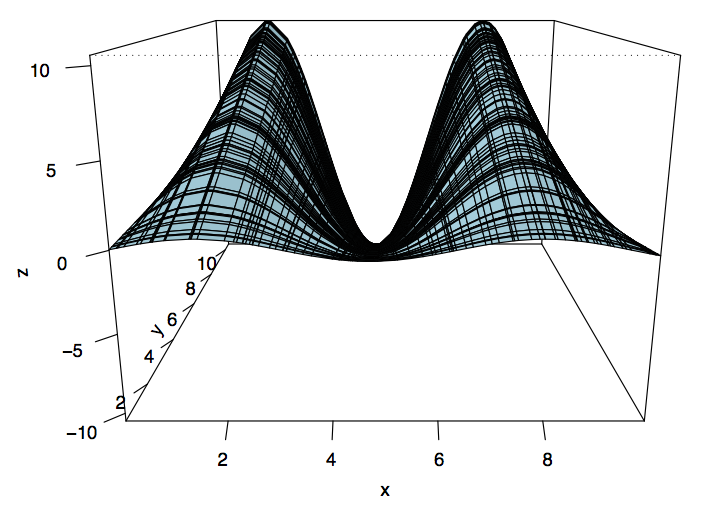
\includegraphics[width = 3.5in]{images/simulation.png}
	\end{center}
   \end{figure}
\end{frame}

%_________
\begin{frame}[fragile]
\frametitle{Simulations}
To visually see its maximum and minimum values, look at the contours of the function:

    \begin{columns}[Tc]
      \column{0.36\textwidth}

\begin{lstlisting}
contour(x,y,z)
\end{lstlisting}

     \column{0.64\textwidth}
   \begin{figure}[ht]
       \begin{center}
		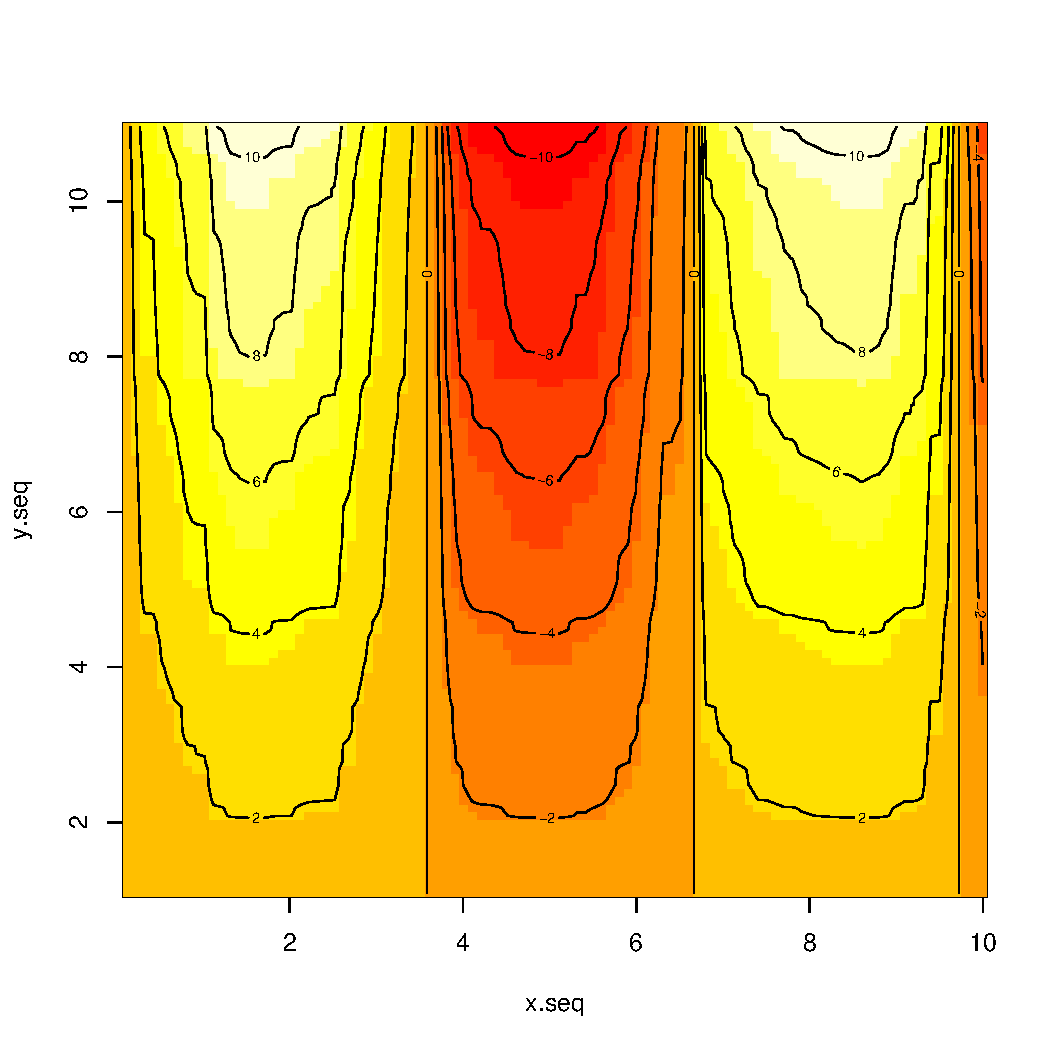
\includegraphics[scale=0.33]{images/contourSim.pdf}
	\end{center}
   \end{figure}
\end{columns}

\end{frame}


%g <- expand.grid(x = 1:10, y = 5:15)
%g$z<-g$x^2
%wireframe(g$z~g$x*g$y, scales = list(arrows = FALSE), drape = TRUE, colorkey = TRUE)


% ------------------------------------------------------------
% ------------------------------------------------------------
\subsection{Exercise V}
\begin{frame}
	\frametitle{Exercise V}
	Visualize the following function:
	\begin{equation}
		z \hspace{0.01in} =\hspace{0.01in} \frac{sin(\frac{3}{2}x)}{y}
	\end{equation}	
\end{frame}

%# Sample from the random uniform:
%x <- sort(runif(100, min=0, max=10))
%y <- x+runif(1)
%f <- function(x,y) { r <- sin(1.5*x)/y}
%z <- outer(x,y,f)
%persp(x, y, z, col = terrain.colors(length(z)/4), shade = 0.1, ticktype = "detailed", expand=0.7)